% !TEX TS-program = pdflatex
% !TEX encoding = UTF-8 Unicode

% This is a simple template for a LaTeX document using the "article" class.
% See "book", "report", "letter" for other types of document.

\documentclass[11pt, preview]{standalone} % use larger type; default would be 10pt

\usepackage[utf8]{inputenc} % set input encoding (not needed with XeLaTeX)


\usepackage{../../markup}
%%% Examples of Article customizations
% These packages are optional, depending whether you want the features they provide.
% See the LaTeX Companion or other references for full information.

%%% PAGE DIMENSIONS
\usepackage{geometry} % to change the page dimensions
\geometry{a4paper} % or letterpaper (US) or a5paper or....
% \geometry{margin=2in} % for example, change the margins to 2 inches all round
% \geometry{landscape} % set up the page for landscape
%   read geometry.pdf for detailed page layout information

\usepackage{graphicx} % support the \includegraphics command and options
\usepackage{color, tikz}
% \usepackage[parfill]{parskip} % Activate to begin paragraphs with an empty line rather than an indent

%%% PACKAGES
\usepackage{amsmath, amsfonts,amssymb}
\usepackage{booktabs} % for much better looking tables
\usepackage{array} % for better arrays (eg matrices) in maths
\usepackage{paralist} % very flexible & customisable lists (eg. enumerate/itemize, etc.)
\usepackage{verbatim} % adds environment for commenting out blocks of text & for better verbatim
\usepackage{subfig} % make it possible to include more than one captioned figure/table in a single float
% These packages are all incorporated in the memoir class to one degree or another...

%%% HEADERS & FOOTERS
\usepackage{fancyhdr} % This should be set AFTER setting up the page geometry
\pagestyle{fancy} % options: empty , plain , fancy
\renewcommand{\headrulewidth}{0pt} % customise the layout...
\lhead{}\chead{}\rhead{}
\lfoot{}\cfoot{\thepage}\rfoot{}

%%% SECTION TITLE APPEARANCE
\usepackage{sectsty}
\allsectionsfont{\sffamily\mdseries\upshape} % (See the fntguide.pdf for font help)
% (This matches ConTeXt defaults)

%%% ToC (table of contents) APPEARANCE
\usepackage[nottoc,notlof,notlot]{tocbibind} % Put the bibliography in the ToC
\usepackage[titles,subfigure]{tocloft} % Alter the style of the Table of Contents
\renewcommand{\cftsecfont}{\rmfamily\mdseries\upshape}
\renewcommand{\cftsecpagefont}{\rmfamily\mdseries\upshape} % No bold!

\newcommand{\N}{\mathbb{N}}
\newcommand{\Prob}{\mathbb{P}}
\newcommand{\E}{\mathbb{E}}
\newcommand{\Z}{\mathbb{Z}}
\newcommand{\R}{\mathbb{R}}
\newcommand{\Q}{\mathbb{Q}}
%%% END Article customizations

%%% The "real" document content comes below...

\date{} % Activate to display a given date or no date (if empty),
         % otherwise the current date is printed 

\begin{document}
\config{name}{Random Variables and Probability Distributions}
\noindent{\bf Random Variables and Probability Distributions.}

\begin{enumerate}
\item {\bf Random Variables.} Consider the following game: you roll two standard 6-sided dice, one after the other. If the number on the first dice divides the number on the second dice, you get 1 point. You get 1 additional point for each prime number you roll.

Define the random variable $R_1$ to be the result of the first roll, and define $R_2$ to be the result of the second roll. Define the random variable $X = R_1 + R_2$ to be the sum of the numbers that come up on both dice, define the random variable $Y = R_1 \cdot R_2$ to be the product of the numbers that come up on both dice, and define the random variable $Z$ to be the number of points you win in the game.

\begin{enumerate}
\item How many values can the random variable $Z$ take on (with nonzero probability)?
\begin{Freeform}{3}
\# values of $Z$ = 
\Hint What are all the possible values of $Z$ as it is defined in this game?
\end{Freeform}
%-----------------------------------------
\item What are the minimum and maximum values that the random variable $Z$ take on  (with nonzero probability)? Please enter your answer in the form $(x,y)$ where $x$ is the minimum value and $y$ is the maximum value (be sure not to use a space!).
\begin{Freeform}{(0,2)}
$(\min Z, \max Z)$ = 
\Hint What are all the possible values of $Z$ as it is defined in this game?
\end{Freeform}
%-----------------------------------------
\item Say that your first roll is a 3 and your second roll is a 6. What is the value of $Z$?
\begin{Freeform}{2}
$Z$ = 
\Hint Review the definition of a random variable--what is the value of this expression given the sample point?
\end{Freeform}
%-----------------------------------------
\item Say that your first roll is a 2 and your second roll is a 1. What is the value of $Z$?
\begin{Freeform}{1}
$Z$ = 
\Hint Review the definition of a random variable--what is the value of this expression given the sample point?
\end{Freeform}
%-----------------------------------------
\item Say that your first roll is a 4 and your second roll is a 1. What is the value of $X^2+Y$?
\begin{Freeform}{29}
$X^2+Y$ = 
\Hint Review the definition of a random variable--what is the value of this expression given the sample point?
\end{Freeform}
%-----------------------------------------
\item Say that your first roll is a 3 and your second roll is a 5. What is the value of $X+Y+2\cdot Z$?
\begin{Freeform}{27}
$X+Y+2\cdot Z$ = 
\Hint Review the definition of a random variable--what is the value of this expression given the sample point?
\end{Freeform}
%-----------------------------------------
\item Conditioned on the fact that your second roll is a 1, what is the probability that $Z = 1$? Please enter your answer as a completely reduced fraction (i.e. in the form $x/y$ where $x,y$ are the smallest possible non-negative integers).
\begin{Freeform}{2/3}
$\Prob[Z = 1|R_2 = 1]$ = 
\Hint Review the definition of a random variable--on how many sample points in the event we are conditioning on does $Z$ take value $1$?
\end{Freeform}
%-----------------------------------------
\item Conditioned on the fact that your second roll is a 1, what is the probability that $Z = 2$?  Please enter your answer as a completely reduced fraction (i.e. in the form $x/y$ where $x,y$ are the smallest possible non-negative integers).
\begin{Freeform}{0/1}
$\Prob[Z = 2 | R_2 = 1]$ = 
\Hint Review the definition of a random variable--on how many sample points in the event we are conditioning on does $Z$ take value $2$?
\end{Freeform}
%-----------------------------------------
\end{enumerate}
%---------------------------------------------------------------------------------------------------------
\item {\bf Distributions of Random Variables.} Match each of the 5 random variables below with the correct probability distribution (of the following choices):

\begin{center}
\begin{tabular}{c|c}
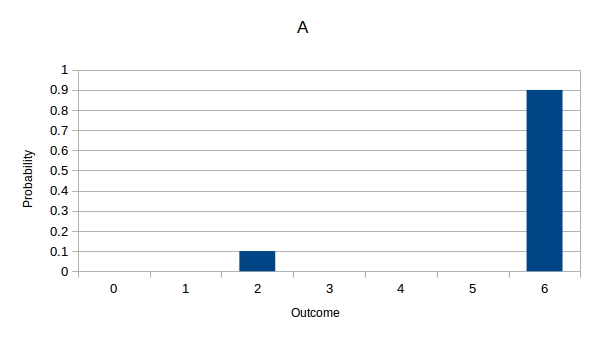
\includegraphics[width=0.4\textwidth]{dists/candy.png} &
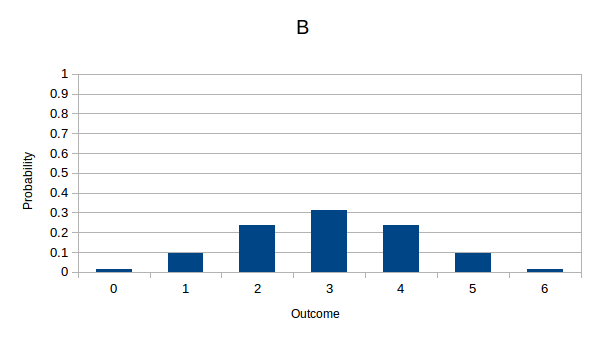
\includegraphics[width=0.4\textwidth]{dists/binom.png}
\\
\hline 
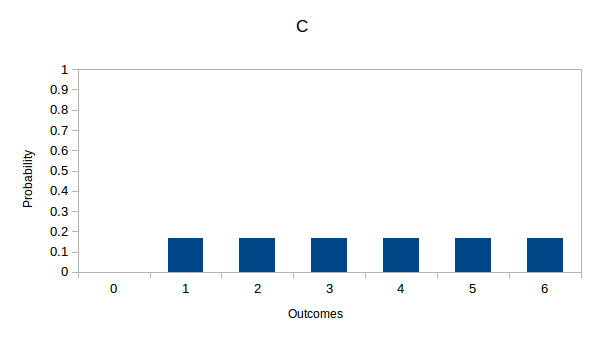
\includegraphics[width=0.4\textwidth]{dists/uniform.png}&
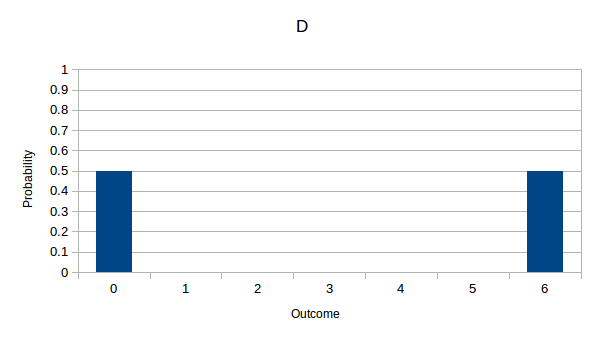
\includegraphics[width=0.4\textwidth]{dists/extreme.png}\\
\hline \vspace{2mm}
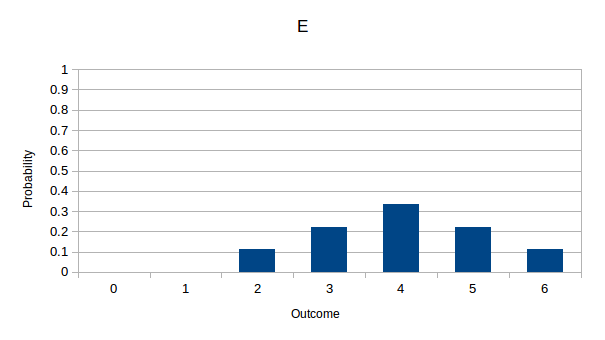
\includegraphics[width=0.4\textwidth]{dists/twodice.png}&
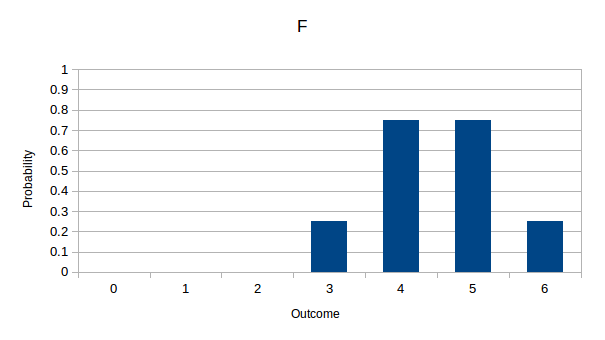
\includegraphics[width=0.4\textwidth]{dists/threeflips.png}\\
\end{tabular}
\end{center}

\begin{enumerate}
%-----------------------------------
\item What is the distribution corresponding to the number of tails, $X$, generated in 6 coinflips?
\begin{Multi}
Review the definition of a random variable and the definition of a probability distribution in note 12.
\begin{itemize}
\FalseChoice\item A
\TrueChoice\item B
\FalseChoice\item C
\FalseChoice\item D
\FalseChoice\item E
\FalseChoice\item F
\end{itemize}
\end{Multi}
%-----------------------------------
\item  What is the distribution corresponding to the outcome $X$ of rolling a standard 6-sided dice?
\begin{Multi}
Review the definition of a random variable and the definition of a probability distribution in note 12.
\begin{itemize}
\FalseChoice\item A
\FalseChoice\item B
\TrueChoice\item C
\FalseChoice\item D
\FalseChoice\item E
\FalseChoice\item F
\end{itemize}
\end{Multi}
%-----------------------------------
\item What is the distribution corresponding to the sum $X_1 + X_2$ of the outcomes of two 3-sided dice, each with sides labeled 1,2,3?
\begin{Multi}
Review the definition of a random variable and the definition of a probability distribution in note 12.
\begin{itemize}
\FalseChoice\item A
\FalseChoice\item B
\FalseChoice\item C
\FalseChoice\item D
\TrueChoice\item E
\FalseChoice\item F
\end{itemize}
\end{Multi}
%-----------------------------------
\item  What is the distribution corresponding to the sum $Z_1 + Z_2 + Z_3$, where $Z_i$ is generated by flipping a coin and setting $Z_i = 2$ if it turns up heads and $Z_i = 1$ if it turns up tails (or, if you like, the sum of three 2-sided dice)?
\begin{Multi}
Review the definition of a random variable and the definition of a probability distribution in note 12.
\begin{itemize}
\FalseChoice\item A
\FalseChoice\item B
\FalseChoice\item C
\FalseChoice\item D
\FalseChoice\item E
\TrueChoice\item F
\end{itemize}
\end{Multi}
%-----------------------------------
\item Say a candy bar is sold for $\$6$ at the corner store, but is sold for $\$2$ at the MegaMart one mile away. Because the MegaMart is 9 times further away than the corner store, you are 9 times more likely to buy the candy bar at the corner store.  What is the distribution corresponding to the price $X$ you pay for the candy bar on a random day (assuming you choose randomly whether to go to the corner store or the MegaMart with probability proportional to the distance).
\begin{Multi}
Review the definition of a random variable and the definition of a probability distribution in note 12.
\begin{itemize}
\TrueChoice\item A
\FalseChoice\item B
\FalseChoice\item C
\FalseChoice\item D
\FalseChoice\item E
\FalseChoice\item F 
\end{itemize}
\end{Multi}
%-----------------------------------
\item When it rains it pours--say that this past April, on half of the days of April there were 0 inches of rain, and the other half of the days there were 6 inches of rain. What is the distribution of $X$, the number of inches of rain on a uniformly random day of April?  
\begin{Multi}
Review the definition of a random variable and the definition of a probability distribution in note 12.
\begin{itemize}
\FalseChoice\item A
\FalseChoice\item B
\FalseChoice\item C
\TrueChoice\item D
\FalseChoice\item E
\FalseChoice\item F
\end{itemize}
\end{Multi}
%-----------------------------------
\end{enumerate}
%---------------------------------------------------------------------------------------------------------
\item {\bf A Preview of Expectations.} Consider a random variable $X$ which takes on values $x_1, \ldots, x_n$. The \emph{expectation} of $X$, denoted $\E[X]$, is defined to be 
\[
\E[X] = \sum_{i = 1}^n x_i \cdot \Prob[X = x_i].
\]
Notice that when $\Prob[X = x_i] = \frac{1}{n}$ for all $i$, then this is simply the familiar notion of an average! You will learn more about the expectation next week, and you can refer to note 12 for more details. For now, we will practice calculating some expectations.

Let us return to the game from the first question: roll two 6-sided dice, award 1 point if the number on the first dice divides the number on the second dice, plus one more point for each prime. Define $R_1$ to be the result of the first roll, define $R_2$ to be the result of the second roll, define $X = R_1 + R_2$ to be the sum of the numbers that come up on both dice, define $Y = R_1 \cdot R_2$ to be the product of the numbers that come up on both dice, and define $Z$ to be the number of points you win in the game.
\begin{enumerate}
\item What is $\E[R_1]$?
\begin{Freeform}{3.5}
$\E[R_1]$ = 
\Hint Review the definition of expectation.
\end{Freeform}
%-----------------------------------------
\item What is $\E[X] = \E[R_1 + R_2]$?
\begin{Freeform}{7}
$\E[X]$ = 
\Hint Review the definition of expectation.
\end{Freeform}
%-----------------------------------------
\item What is $\E[2\cdot R_1]$? What do you notice about this expectation?
\begin{Freeform}{7}
$\E[X]$ = 
\Hint Review the definition of expectation.
\end{Freeform}
%-----------------------------------------
\item What is $\E[Z | R_2 = 1]$, the expected number of points we win conditioned on the fact that the second dice roll is a 1? Please enter your answer as a completely reduced fraction (i.e. in the form $x/y$ where $x,y$ are the smallest possible positive integers).
\begin{Freeform}{2/3}
$\E[Z | R_2 = 1]$ = 
\Hint Review the definition of expectation--here, we are only considering expectation over the sample points in which $R_2 = 1$.
\end{Freeform}
%-----------------------------------------
\end{enumerate}

% --------------------------------------------------------------------------------------------------------------------------
\item {\bf Binomial Games} Suppose that the Cleveland Browns have probability $p = 0.15$ chance of winning a football game. Assume that the results of all games are mutually independent. The football regular season has 16 games.
\begin{enumerate}
    \item Write an expression for the probability that they win between $6$ and $8$ games (inclusive) during the course of a season. Evaluate it and round it to the 2nd decimal place.
    \begin{Freeform}{0.02}
    \Solution \[\binom{16}{6}(0.15)^6(0.85)^{10} + \binom{16}{7}(0.15)^7(0.85)^9 + \binom{16}{8}(0.15)^8(0.85)^8\]
    \end{Freeform}

    \item Find the probability that they win at least one game during the course of a season. Round your answer to the 2nd decimal place
    \begin{Freeform}{0.92}
    \Solution We could sum up the probabilities that they win 1 game, 2 games, etc. or, we could find the probability that they win 0 games and subtract that from 1. \[p = 1 - 0.85^{16} = .92\]
    \end{Freeform}
\end{enumerate}
% --------------------------------------------------------------------------------------------------------------------------
\item {\bf Absent Cal Bear} Andy is a freshman at Cal. Every day, Andy wakes up, silences his 7:30 alarm, and chooses whether to go to class or back to sleep. With $p = 0.2$ he chooses to go to class, and with probability $0.8$ he decides otherwise. His choices on each day are mutually independent. Find probabilities of the following events:
\begin{enumerate}
    \item the first time he goes to class is the $5^{th}$ day of school?
    \begin{Choices}
    \begin{itemize}
    	\TrueChoice\item $(1-0.2)^40.2$
    	\FalseChoice\item $0.2^4(1-0.2)$
    	\FalseChoice\item $(1-0.2)^4$
    	\FalseChoice\item $0.2^5$
    \end{itemize}
    \Solution $(1-0.2)^40.2$
    \end{Choices}

    \item the first time he goes to class is after the $5^{th}$ day? Round your answer to the 2nd decimal place.
    \begin{Freeform}{0.33}
    \Solution Let $X \sim Geom(n,p)$. \[ p = \sum_{i = 5}^{\infty} (1-0.2)^{i}0.2\] We can solve this using the sum of an infinite geometric series.

    We can also consider the following approach: in order for him to go to class for the first time after the $5^{th}$ day, all he has to do is fail to go to class for 5 days in a row. This probability is $(1-0.2)^5 = 0.33$. 

    To see that the two approaches agrees, we have in general: $P(X>k) = \sum_{i=k + 1}^{\infty} P(X=i) = \sum_{i=k}^{\infty} p(1-p)^i = p(1-p)^k - \sum_{i=0}^{\infty} (1-p)^i = p(1-p)^k \frac{1}{1-(1-p)} = (1-p)^k$.
    \end{Freeform}

    \item He goes to class on the $5^{th}$ day or before? Round your answer to the 2nd decimal place.
    \begin{Freeform}{0.67}

    \Solution Use the complement of the last question. $p = 1-(1-0.2)^5 = 0.67$. In general: $P(X\leq k) = 1-(1-p)^k$.  
    \end{Freeform}

\end{enumerate}

% --------------------------------------------------------------------------------------------------------------------------
\item {\bf Alternating Darts} Alex and Bob are playing darts. They take turns throwing the dart and the first one to hit the center wins. Each turn, Alex hits the center with probability $p$ and Bob hits the center with probability $q$. Alex gets to go first. We will explore two ways of finding out how likely it is for Alex to win.

\begin{enumerate}
    \item What is the probability that Alex wins on the $k^{th}$ turn? 
    \begin{Choices}
    \begin{itemize}
    	\FalseChoice\item $(1-p)^{k-1}p$
    	\FalseChoice\item $(1-p)^{k-1}q^kp$
    	\TrueChoice\item $((1-p)(1-q))^{k-1}p$
    	\FalseChoice\item $((1-p)(1-q))^{k-1}pq$
    \end{itemize}
    \Solution both Alex and Bob must miss for the first $k-1$ turns, then Alex must hit the center on the $k^{th}$ turn. Thus, the probability he wins on the $k^{th}$ turn is $((1-p)(1-q))^{k-1}p$
    \end{Choices}


    \item Denote the answer from the previous part $p_k$. What is the probability that Alex wins on any turn? Select all that apply
    \begin{Multi}
    \begin{itemize}
    	\FalseChoice\item $\frac{p}{p+q}$
    	\TrueChoice\item $\frac{p}{p+q-pq}$
    	\TrueChoice\item $\sum_{k=1}^{\infty} p_k$
    	\FalseChoice\item $\Pi_{k=1}^{\infty} p_k$
    \end{itemize}
    \Solution Let $A_k$ denote the event that Alex won on turn $k$.
    $$\sum_{k=1}^{\infty} P(A_k) = \sum_{k=1}^{\infty}((1-p)(1-q))^{k-1}p = p\sum_{k=0}^\infty((1-p)(1-q))^{k} = \frac{p}{1-(1-p)(1-q)} = \frac{p}{p+q-pq} $$
    \end{Multi}
    

    \item we say that the game ended on turn $k$ if either Alex or Bob hit the center on turn $k$. Let $X$ be a random variable corresponding to the turn that the game ended on. What is the distribution of $X$?
    \begin{Choices}
    \begin{itemize}
    	\FalseChoice\item $Binom(p+q-pq)$
    	\FalseChoice\item $Binom(p)$
    	\FalseChoice\item $Binom(p(1-q))$
    	\FalseChoice\item $Geom(p)$
    	\TrueChoice\item $Geom(p+q-pq)$
    	\FalseChoice\item $Geom(p(1-q))$
    \end{itemize}

    \Solution The probability that the game ends on each turn equals to the probability that either Alex or Bob hits the center on that turn, and each turn is independent. By the inclusion-exclusion principal, the probability that either Alex or Bob hits the center on a given turn is $p+q-pq$. Thus $X \sim Geom(p+q-pq)$. 

    Alternative approach: Let $Y$ be the random variable indicating the number of turns it takes for Alex to hit the center. So $Y \sim Geom(p)$. Define $Z$ similarly for Bob and so $Z \sim Geom(q)$. Since the game ends on the turn when either of them hits the center, we know $X = min(Y, Z)$. From discussion, we know $X = min(Y, Z) \sim Geom(p + q - pq)$. This agrees with our previous approach. 
    \end{Choices}
    

    \item  Using parts $a$ and $c$, what is the probability that Alex wins given that the game ended on turn $k$? Select all that apply. 
    \begin{Multi}{}
    \begin{itemize}
    	\FalseChoice\item $\frac{p}{p+q}$
    	\TrueChoice\item $\frac{p}{p+q-pq}$
    	\TrueChoice\item $\frac{((1-p)(1-q))^{k-1}p}{((1-p)(1-q))^{k-1}(p+q-pq)}$
    	\FalseChoice\item $\frac{((1-p)(1-q))^{k-1}p}{((1-p)(1-q))^{k-1}(p+q)}$
    \end{itemize}
    \Solution Let $A_k$ denote the event that Alex won on turn $k$. Then we have
        \begin{align*}
            Pr[A_k | X=k] &= \frac{Pr[A_k \cap X=k]}{Pr[X=k]}\\
            &= \frac{Pr[A_k]}{Pr[X=k]}\\
            &= \frac{((1-p)(1-q))^{k-1}p}{((1-p)(1-q))^{k-1}(p+q-pq)}\\
            &=\frac{p}{p+q-pq}
        \end{align*}

    \end{Multi}
    
\end{enumerate}

% --------------------------------------------------------------------------------------------------------------------------


\end{enumerate}
\end{document}
